\documentclass[]{../../math_paper}
\usepackage[margin=0.5in]{geometry}

\title{Finding Shortest Paths Using Tropical Linear Algebra}

\author{Kazuya Erdos}

%%%%%%%%%%%%%%%%%%%%%%%%%%%%%%%%%%%%%%%%%%%%%%%%%%%%%%

\title{The Group Law of Elliptic Curves}

\begin{document}
\maketitle

\begin{abstract}
    Elliptic curves are of the form $y^2 = x^3 + ax + b$. In this paper we give their history and prove a group law on the points of an elliptic curve. To add two points on the curve, we draw the line through them and reflect its intersection point with the curve over the $x$-axis. We also motivate the projective plane and a point "at infinity" that must be included as the identity element for this group. We apply this group law to cryptographic systems, utilizing the extreme difficulty of knowing how many times a point was added to itself to yield another point.
\end{abstract}
\section{Introduction}
Elliptic curves are one of the most studied objects in mathematics---they have numerous applications in modern cryptography and played a pivotal role in proving Fermat's Last Theorem, one of the oldest and most famous problems in history. Elliptic curves are defined over a field $K$ as $y^2 = x^3 + ax + b$. Amazingly, if we add add a point "at infinity," called $\mathcal{O}$ to the set of points on an elliptic curve $E(K)$, then we are able to form an Abelian group with a surprisingly intuitive operation. To add points $P$ and $Q$, we simple take the third point of intersection with the curve and the line formed by $P$ and $Q$, and reflect over the $x$-axis. This is known as "chord and tangent addition," and is stated formally in Theorem \ref{thm:main}:

\begin{maintheorema}
    The binary operation $+$ defined in Algorithms \ref{grouplaw} and \ref{geometric} endows the set $E(K)$ with an Abelian group structure, with identity $\mathcal{O}$.
\end{maintheorema}

\begin{example}
    Let $E(\Q) \cup \{\mathcal{O}\}$ be the group law over the elliptic curve $y^2 = x^3 - 5x + 45$. Figure \ref{fig:curve1} shows $(1, 0) + (0, 2) = (3, 4)$ over $E(\Q) \cup \{\mathcal{O}\}$, which follows chord and tangent addition nicely. Let $E(\Z/37\Z) \cup \{\mathcal{O}\}$ be the gropu law over the elliptic curve $y^2 = x^3 + x$. Figure \ref{fig:curve2} shows $(10, 14) + (24, 26) = (24, 11)$ over $E(\Z/37\Z) \cup \{\mathcal{O}\}$, which is less intuitive.
\end{example}

\begin{figure}[H]
    \centering
    \begin{minipage}{.5\textwidth}
        \centering
        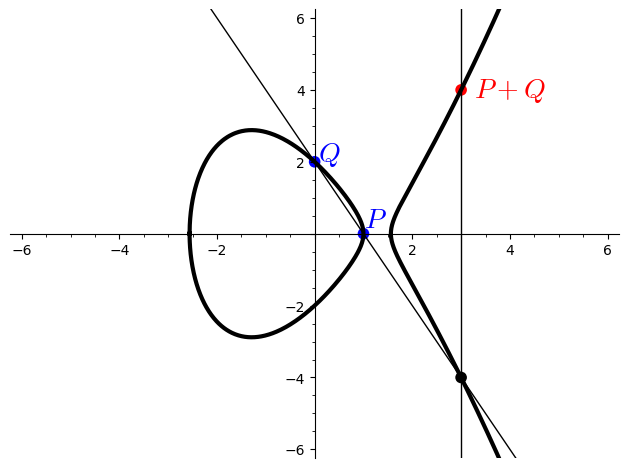
\includegraphics[height = 2 in]{media/curve_1.png}
        \captionof{figure}{A visualization of the chord and tangent addition of points $(1, 0) + (0, 2) = (3, 4)$ over $E(\Q) \cup \{\mathcal{O}\}$}
        \label{fig:curve1}
    \end{minipage}%
    \begin{minipage}{.5\textwidth}
        \centering
        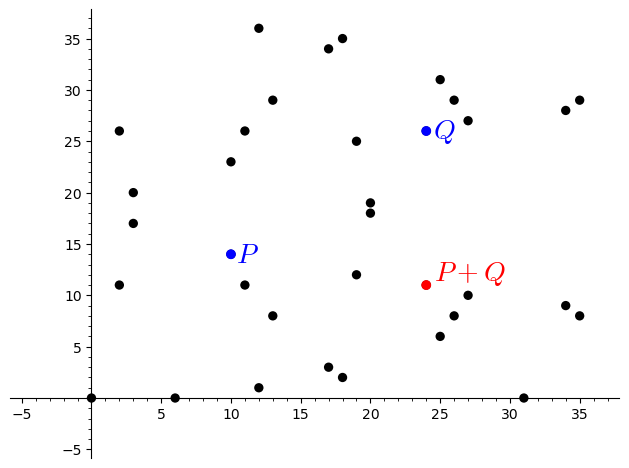
\includegraphics[height = 2 in]{media/curve_2.png}
        \captionof{figure}{A less intuitive visualization of the addition of points $(10, 14) + (24, 26) = (24, 11)$ over $E(\Z/37\Z) \cup \{\mathcal{O}\}$}
        \label{fig:curve2}
    \end{minipage}
\end{figure}

Why are elliptic curves given their name? It is a common mistake to assume that the curves are in related in shape to ellipses, though they do indeed share a loose history. Traces of Theorem \ref{thm:main} were around as early as the $17^{\text{th}}$ century, when Fermat and Bachet developed algebraic formulas to add points on cubic curves with chords and tangents \cite{rice}, though their methods were not formalized until many years later. In a 1738 paper, Leonard Euler discovered a method to find the arc length of an ellipse \cite{sandifer2007euler}. It turned out that while finding the arc length of a circle was trivial, it took a great deal of effort to derive equations for the arc length of ellipses. His solution involved taking complicated integrals, which were later generalized to be known as \emph{elliptic integrals}. Building upon Euler's work, Adrien-Marie Legendre was able to adapt   the integrals into functions of their upper bounds, something he called \emph{elliptic functions}. Legendre was able to apply these functions to the motion of a simple pendulum \cite{legendre}. Legendre's elliptic functions, however, are not the same elliptic functions that we know of today.

In 1827, both Carl Gustav Jacob Jacobi and Niels Henrik Abel indepedently discovered a way to invert elliptic integrals by viewing their upper bounds as functions of the integrals over the complex plane\cite{jacobi1829fundamenta} \cite{abel}. These are what are known today as \emph{elliptic functions}. Jacobi believed that Legendre missed this revelation since he was not very comfortable with complex numbers, which were a budding branch of mathematics at the time. At last, in 1864, Alfred Clebsch used the elliptic functions to parameterize cubic curves, coining the term \emph{elliptic curve}. Soon after, Karl Weiertrass was able to link an addition formula for elliptic functions to elliptic curves. Finally, in 1901 Henri Poincare tied together all of the ideas, rigorously proving the group law of Theorem \ref{thm:main} over chord and tangent addition\cite{H1901}.

Elliptic Curves have numerous and surprising applications. In 1957, Yutaka Taniyama and Goro Shimura devised the Taniyama-Shimura conjecture, which stated that elliptic curves over the rational numbers are related to modular forms, a seemingly separate mathematical object. This conjecture, now adapted and proven as the \emph{modularity theorem}, was privotal for Andrew Wiles and Richard Taylor to prove Fermat's Last Theorem, one of the oldest and most famous theorems in mathematics (for more on this exciting story, see \cite{singh1998fermat}). The group law of elliptic curves described in Theorem \ref{thm:main} can be applied to construct modern cryptosystems. In fact, elliptic curves provide strong security while using smaller key sizes than the industry standard RSA cryptosystem \cite{stein2008elementary}.

The strucutre of the paper is as follows: In Section \ref{sec:background} we the define the key ingredients needed for understanding elliptic curves and Theorem \ref{thm:main}; in Section \ref{sec:thm} we prove Theorem \ref{thm:main}; in Section \ref{sec:applications} we discuss an application of cryptography; in Section \ref{sec:future} we give the reader further areas of study.

\subsection*{Acknowledgements}
I would like to thank Professor Madeline Brandt for teaching me Abstract Algebra and always being responsive to questions. I would also like to thank Tanish Makadia for listening to me ramble on and on about these funny curves.
\section{Background} \label{sec:background}
We assume that the reader is familiar with groups, fields, and polynomials.

\begin{definition} (Elliptic Curve) \cite{stein2008elementary}. An \emph{elliptic curve} over a field $K$ is a curve defined by an equation of the form
    $$y^2 = x^3 + ax+ b$$
    Where $a, b \in K$ and $-16(4a^3 + 27b^2) \neq 0$. The descriminant $\Delta = -16(4a^3 + 27b^2)$ is required to be nonzero so that the curve has no cusps, self-intersections, or isolated points. To learn more about this condition, see \cite{Silverman:1338326}.
\end{definition}

\subsection{The Projective Plane and Points at Infinity}
We will find that in order to place a group structure on elliptic curves, we will need to move into a \emph{projective plane}. We would like for every pair of distinct lines to intersect at exactly one point. Clearly, over the regular plane (called the \emph{affine plane}), parallel lines never intersect. So, we will need to add a collection of "points at infinity" to the regular plane \cite{Fitchett}.

Consider the lines $y = x$ and $y = x + 1$. Since these lines are parallel, we will have to add a point at infinity at which they will intersect. For $y = 2x$ and $y = 2x + 1$, we will have to add another point at infinity for them to intersect. This second point cannot be the same point as the first point we added, beacuse then $y = x$ and $y = 2x$ would intersect at \emph{both} that point and at the origin, which breaks our rule of distinct lines intersecting at exactly one point. Continuing this logic, we find that we need one point at infinity for each possible slope of a line.

From this, we can develop a new coordinate system in the projective plane. We denote points $(x, y)$ in the regular plane as $[x, y, 1]$. We denote points at infinity which intersect lines with slope $y/x$ as $[x, y, 0]$. Note that vertical lines contain the point $[0, 1, 0]$. Of course, now that our points have three coordinates, we need three variables. This is outside the scope of this article, but see \cite{Fitchett} to learn more about a process called \emph{homogenization} wherein curves over the regular plane can be homogenized to functions of three variables.

With our new understanding of the projective plane, we can now tackle Bézout's Theorem, which will be critical for proving Theorem \ref{thm:main}.

\begin{theorem} (Bézout's Theorem) \cite{Fitchett}. If $C$ and $D$ are complex projective (algebraic) curves that do not have an infinite number of points in common (for example when $C$ = $D$), then \begin{equation*}
        \sum_{P \in C \cap D}i(C \cap D, P) = (\mathrm{deg}C)(\mathrm{deg}D)
    \end{equation*}
    where $i(C \cap D)$ is the number of times $C$ and $D$ intersect at point $P$, called the intersection multiplicity of $P$ \cite{nichols2013intersection}.
\end{theorem}

So, Bézout's Theorem tells us that the number of intersection points, when accounding for multiplicity, between two curves is the product of their degrees.
\begin{definition} The point $\mathcal{O}$ of an elliptic curve $E$ is the point on the curve "at infinity." Using the projective plane coordinate system, it is located at $[0, 1, 0]$.
\end{definition}

So, $\mathcal{O}$ is the point that intersect every vertical line in the projective plane. With our elliptic curve and $\mathcal{O}$, we construct a set that we can put an Abelian group structure on:

\begin{definition} (Candidate Group Structure of Elliptic Curves). Let $E$ be an elliptic curve over the field $K$, given by the equation $y^2 = x^3 + ax + b$. Then
    $$E(K) = \{(x, y) \in K \oplus K \mid y^2 = x^3 + ax + b\} \cup \{\mathcal{O}\}$$
\end{definition}

We will discover that $\mathcal{O}$ will act as the identity element in this group. We can then define a binary operation $+$ on $E(K)$ both algebraically and geometrically:

\begin{algorithma} \label{grouplaw} (Algebraic Elliptic Curve Group Law) \cite{stein2008elementary}. Given $P_1, P_2 \in E(K)$, this algoirithm computes a third point $R = P_1 + P_2 \in E(K)$:
    \begin{enumerate}
        \item If $P_1 = \mathcal{O}$, then set $R = P_2$ and terminate. If $P_2 = \mathcal{O}$, then set $R = P_2$ and terminate. Otherwise set $P_1 = (x_1, y_1)$ and $P_2 = (x_2, y_2)$.
        \item If $x_1 = x_2$ and $y_1 = -y_2$, set $R = \mathcal{O}$ and terminate.
        \item Set $\lambda = \begin{cases} (3x_1^2 + a) / (2y_1) & \text{if $P_1 = P_2$} \\ (y_1 - y_2)/(x_1 - x_2) & \text{otherwise} \end{cases}$
        \item Set $R = (\lambda^2 - x_1 - x_2, -\lambda x_3 - \nu)$, where $\nu = y_1 - \lambda$ and $x_3 = \lambda^2 - x_1 - x_2$ is the $x$-coordinate of $R$.
    \end{enumerate}
\end{algorithma}

The algebraic setup for the operation should not be focused on too heavily, since the geometric interpretation of addition (chord and tangent addition) is much more elegant and easy to visualize.
\begin{algorithma} \label{geometric} (Geometric Elliptic Curve Group Law)
    To find the sum $P_1 + P_2$, we find the third point $P_3$ of intersection between $E$ and the line $L$ determined by $P_1$ and $P_2$. The sum $P_1 + P_2$ is the reflection of $P_3$ about the $x$-axis \cite{stein2008elementary}. We know that this third point $P_3$ exists in the projective plane by Bézout's Theorem. The process is similar for adding a point to itself, except we take the tangent line through that point instead. For an explanation of how the algebraic and geometric interpretations are equivalent, see \cite{Kline}.
\end{algorithma}

Figures \ref{fig:curve1} and \ref{fig:curve3} demonstrate simple chord and tangent addition. In Figure \ref{fig:curve3} it is clear that the tangent line drawn through $P$ intersects the curve at $\mathcal{O}$, thus $P + P = \mathcal{O}$.

\begin{figure}[H]
    \centering
    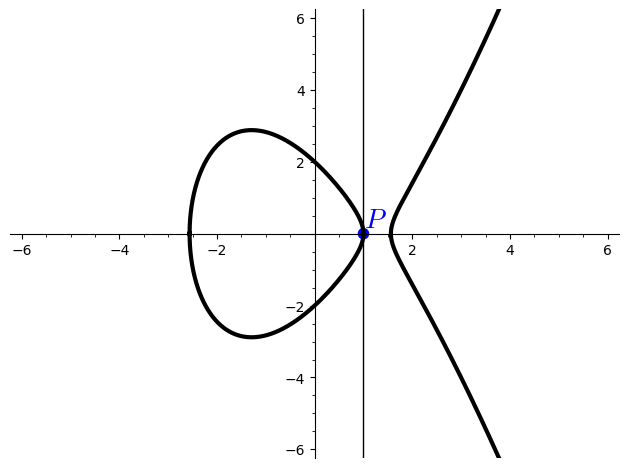
\includegraphics[height = 2in]{media/curve_3.png}
    \captionof{figure}{Visualization of $(1, 0) + (1, 0) = \mathcal{O}$ on some $E(\Q) \cap \{\mathcal{O}\}$}
    \label{fig:curve3}
\end{figure}

We can now move to our main result.
\section{Main Theorem} \label{sec:thm}
\begin{maintheorem}(As given in \cite{stein2008elementary}):
    \label{thm:main}
    The binary operation $+$ defined in Algorithms \ref{grouplaw} and \ref{geometric} endows the set $E(K)$ with an Abelian group structure, with identity $\mathcal{O}$.
\end{maintheorem}
We will verify that $+$ satisfies the axioms of an abelian group with identity $\mathcal{O}$:
\begin{enumerate} [label = (\roman*)]
    \item For all $P \in E(K)$, $P + \mathcal{O} = P$.
    \item For all $P \in E(K)$, there exists $P' \in E(K)$ such that $P + P' = \mathcal{O}$
    \item For all $P, Q \in E(K)$, $P + Q = Q + P$.
    \item For all $P, Q, R \in E(K)$, $P + (Q + R) = (P + Q) + R$.
\end{enumerate}
\begin{proof} We verify each axiom.
    \begin{enumerate} [label = (\roman*)]
        \item Consider $P + \mathcal{O}$. By the definition of $\mathcal{O}$, the line that goes through $P$ and $\mathcal{O}$ is the vertical line that goes through $P$. By Bézout's Theorem, this vertical line must also intersect $E$ at a third point $P'$. This is the point on $E$ that is the reflection of $P$ across the $x$-axis. So, to obtain $P + \mathcal{O}$, we construct the vertical line through $P$ and $\mathcal{O}$, find the third intersection point $P'$, then reflect $P'$ across the $x$-axis, meaning that $P + \mathcal{O} = P.$ This also follows from step $1$ of \ref{grouplaw}.
        \item Let $P = (x_1, y_1), P' = (x_1, -y_1) \in E(K)$ From step $2$ of \ref{grouplaw}, it is immediately clear that $P$ and $P'$ are inverses, since $(x_1, y_1) + (x_2, y_2) = \mathcal{O}$.
        \item Let $P, Q \in E(K)$. $P + Q$ is determined by the line that goes thorugh $P$ and $Q$. This is clearly the same line that goes through $Q$ and $P$. So, $P + Q = Q + P$.
        \item Proving associativity is rather difficult. See \cite{fujii} for an algebraic proof of associativity. To prove associativity graphically, we will need a lemma which encorporates Bézout's Theorem:
              \begin{lemma} \label{lem}
                  If $P_1, \ldots, P_8$ are points in a projective plane, no $4$ on a line, no $7$ on a conic, then there exists a $9^{\text{th}}$ point $Q$ such that a cubic through $P_1, \ldots, P_8$ also passes through $Q$.
              \end{lemma}
              The proof for Lemma \ref{lem} can be found in \cite{cassels_1991}. We wish to show that for $A, B, C \in E(K)$, we have $$(A + B) + C = A + (B + C)$$
              So, it is sufficient to show that
              $$-((A + B) + C ) = -(A + (B + C))$$
              We construct the following lines:
              \begin{align*}
                  L_1 & \quad \text{is the line through}  & A,\qquad      & B,           & -(A + B)       \\
                  L_2 & \quad \text{is the line through}  & A + B, \qquad & C,           & -((A + B) + C) \\
                  L_3 & \quad  \text{is the line through} & B + C, \qquad & \mathcal{O}, & -(B + C)       \\
                  N_1 & \quad \text{is the line through}  & A + B,\qquad  & \mathcal{O}, & -(A + B)       \\
                  N_2 & \quad \text{is the line through}  & B, \qquad     & C,           & -(B + C)       \\
                  N_3 & \quad \text{is the line through}  & A, \qquad     & B+C,         & -(A + (B + C))
              \end{align*}
              Figure \ref{fig:grid1} shows a drawing of the lines and points, adding a point $D$ as the single point of intersection of $L_2$ and $N_3$.

              \begin{figure}[H]
                  \centering
                  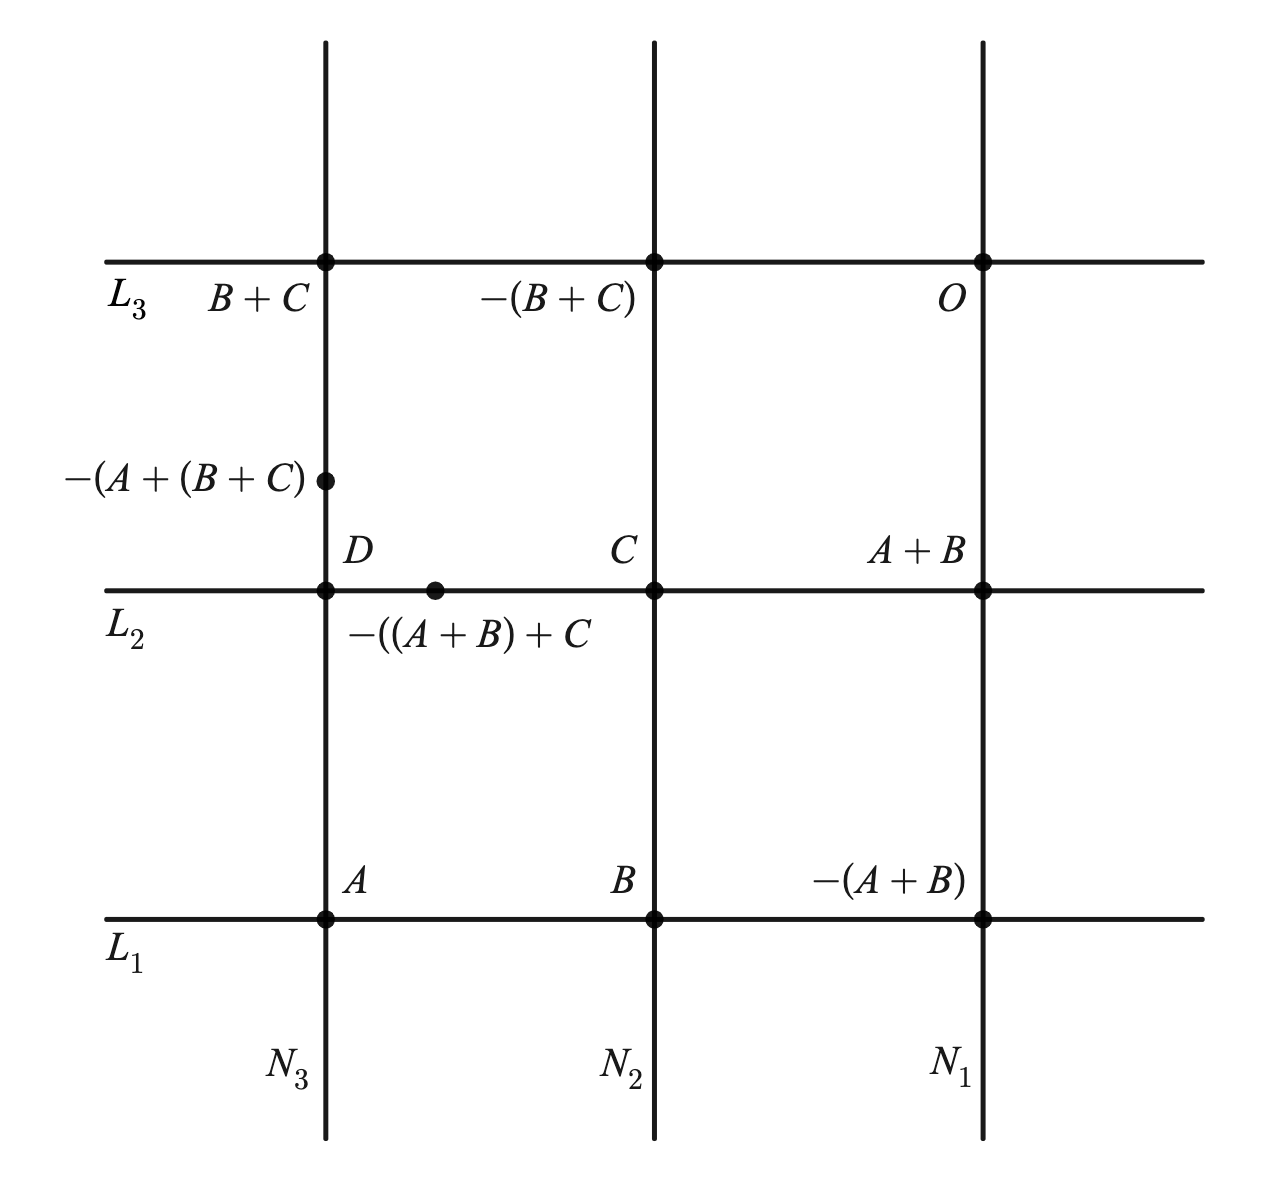
\includegraphics[height = 3in]{media/grid_1.png}
                  \captionof{figure}{A construction of lines in projective space}
                  \label{fig:grid1}
              \end{figure}

              This drawing is meant to keep track of the intersection points, and is not accurate. As a reminder, in Figure \ref{fig:grid2} we sketch our elliptic curve passing through all of the points except for $D$ (we wish to prove that it passes through $D$).

              \begin{figure}[H]
                  \centering
                  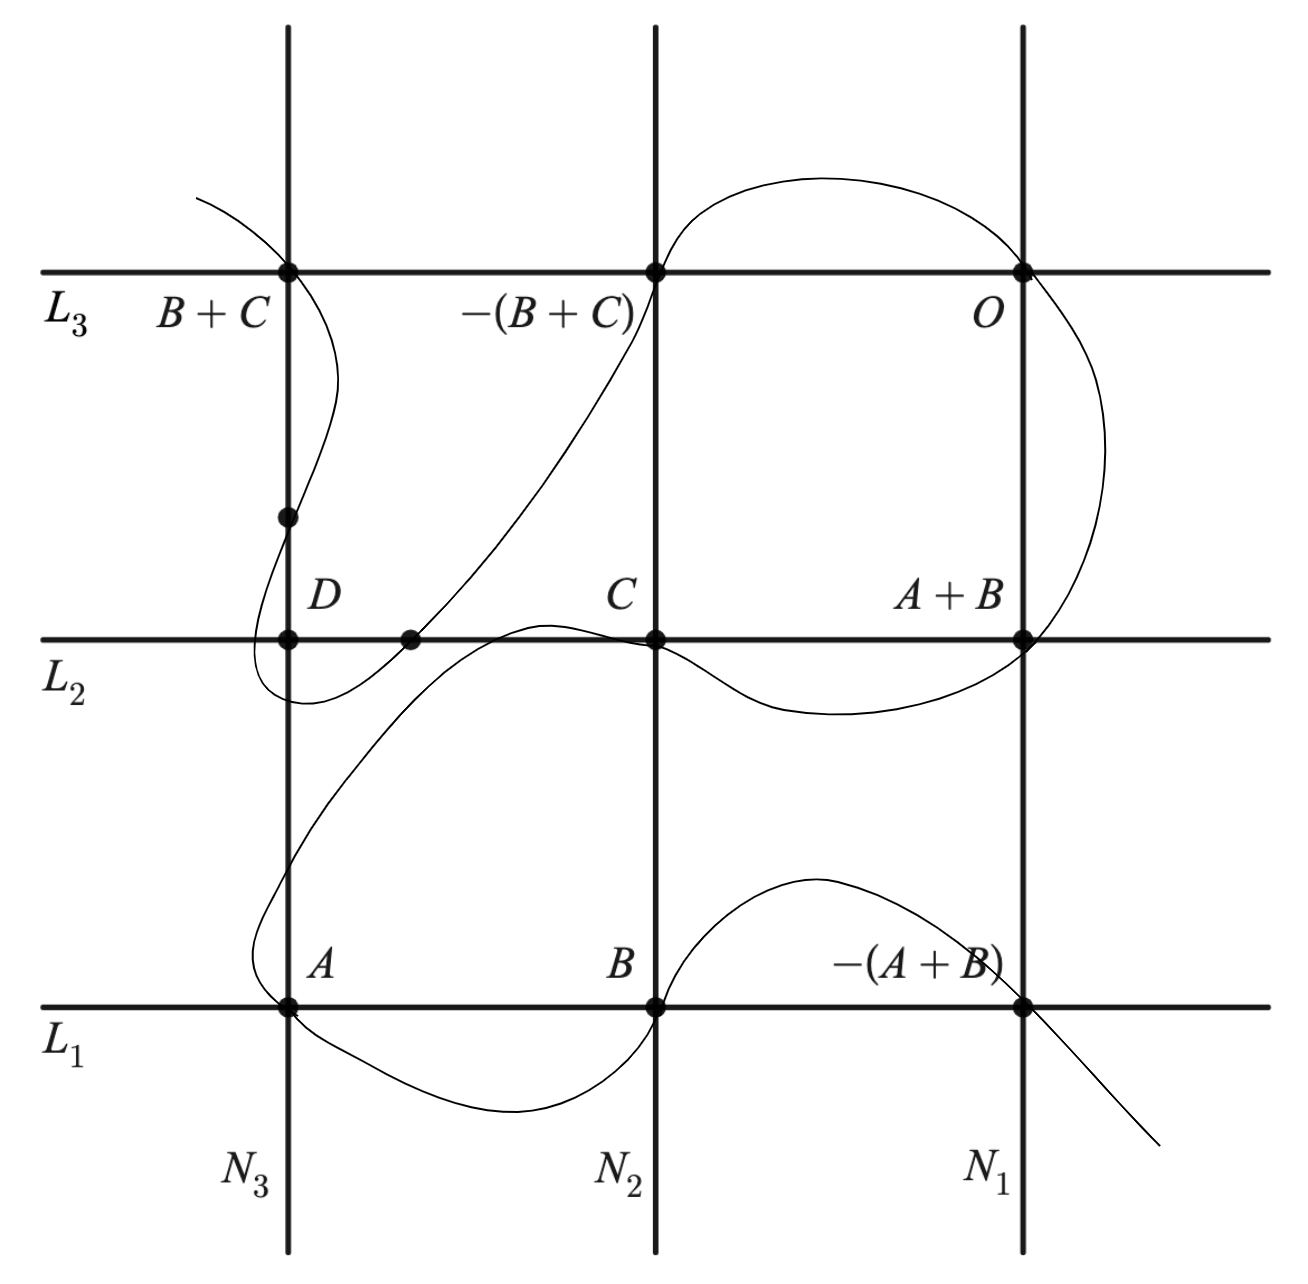
\includegraphics[height = 3in]{media/grid_2.png}
                  \captionof{figure}{The same construction of lines with the elliptic curve drawn in the background}
                  \label{fig:grid2}
              \end{figure}

              From their definitions, we know that $-((A + B) + C)$ lies on $L_2$, and $-(A + (B + C))$ lies on $N_3$. We wish to show that both of these points are equal to $D$. We have the two cubic curves
              $$(L_1L_2L_3)= 0 \qquad \text{and} \qquad (N_1N_2N_3) = 0$$
              By construction, both of these curves pass through the $8$ points
              $$\mathcal{O}, \quad A, \quad B, \quad C, \quad A + B, \quad B + C, \quad -(A + B), \quad -(B + C)$$
              By Bézout's Theorem, we know that the two cubics intersect in $3 \cdot 3 = 9$ points, and we call the $9^{\text{th}}$ point $D$. By the lemma (we will show the conditions are satisfied after), we know that any other cubic through these $8$ points also passes through $D$. So, since $E$ is through these $8$ points, $E$ also passes through $D$ On $N_1N_2N_3 \cap E(K)$ we have the points
              $$\mathcal{O}, A, B, C, A+B, B+C, -(A + B), -(B + C), -(A + (B+C)), D$$
              However, by Bézout's Theorem there must be only $3 \cdot 3 = 9$ points on $N_1N_2N_3 \cap E(K)$, so two of these points must be equal. By construction $D$ is not equal to any of the first $8$ points, so we have that
              $$D = -(A + (B + C))$$
              By the same process, if we consider the $10$ labeled points on $L_1L_2L_3 \cap E$, we will find that $D = -(A + (B + C))$. So,
              $$-(A + (B + C)) = D = -((A + B) + C),$$
              and so this completes the proof for associativity.

              We now show that the lemma does apply. No four of the points
              $$\mathcal{O}, \quad A, \quad B, \quad C, \quad A + B, \quad B + C, \quad -(A + B), \quad -(B + C)$$
              can lie on a line, since if those four points are on a line $L$, then since they are also on $E$, we have that $$\sum_{P \in L \cap E}i(L \cap E, P) \geq 4$$
              which contradicts Bézout's Theorem since a line and a cubic can intersect at at most $1 \cdot 3 = 3$ points. Also, no $7$ of the points can lie on a conic $C$, since they are also on $E$, so
              $$\sum_{P \in C \cap E}i(C \cap E, P) \geq 7$$
              which also contradicts Bézout's Theorem since a conic and a cubic can intersect at at most $2 \cdot 3 = 6$ points. So, the lemma does apply.
    \end{enumerate}
    So, we have satisfied all of the Abelian group axioms, thus the proof is complete.
\end{proof}
\begin{example}
    Three collinear points in $E(K)$ sum to $\mathcal{O}$.
\end{example}
This result follows from the definition of the group law. Let $P, Q, R \in E(K)$ be collinear points. By definition, $P + Q$ is the reflection across the $x$-axis of the intersection point, $R'$, of the line defined by $P$ and $Q$ and $E(K)$. Since $P, Q$ and $R$ are collinear, then $R$ must equal $R'$. Then $P + Q$ is the reflection across the $x$-axis of $R$, which implies that $P + Q$ is the inverse of $R$. So, we have that $P + Q + R = \mathcal{O}$, as desired. Figure \ref{fig:curve4} visualizes this consequence of the group law.

\begin{figure}[H]
    \centering
    \captionsetup{justification=centering}
    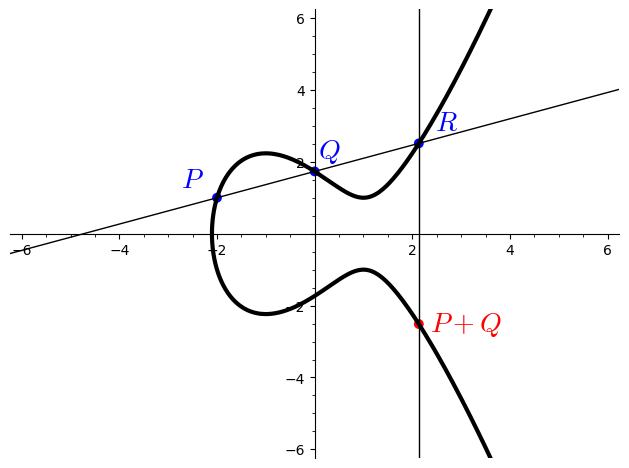
\includegraphics[height = 2in]{media/curve_4.png}
    \captionof{figure}{A visualization of the addition of three collinear points on the elliptic curve $E(\Q)$ given by $y^2 = x^3 - 3x + 3$}
    \label{fig:curve4}
\end{figure}

\section{Elliptic-Curve Diffie-Helman (ECDH)} \label{sec:applications}
In cryptography, elliptic curves are used to generate private keys. These keys are large numbers used as a means to encrypt data sent between two parties.
\\

\noindent\textbf{Original Example.} Suppose that Alice and Bob wished to generate a private key to send encrypted text messages. They would agree on some parameters:
\begin{enumerate}
    \item $p$, a large prime
    \item $E(\Z/p\Z)$: an elliptic curve over $\Z/p\Z$
    \item $G$: a generator point on the curve
    \item $n$: a sufficiently large number
    \item $d_A, d_B$: the private keys for Alice and Bob. These are random integers in $[1, n - 1]$. Importantly, \emph{only} Alice and Bob known their respective private keys. These are never shared or sent publically.
\end{enumerate}

Suppose that Alice and Bob choose the curve $y^2 = x^3 + x - 3$ over the field $\Z/563Z$. Note that in standard practice curves with much larger coefficients and values of $p$ are used \cite{stein2008elementary}. Suppose they chose the generator $(163, 263)$, Alice set $d_A = 13410$, and Bob set $d_B = 43191$. Using the group law described in Theorem \ref{thm:main}, Alice calculates the point $Q_A = d_A \cdot G = (528, 188)$, and Bob calcualtes $Q_B = d_B \cdot G = (337, 318)$ (here $\cdot$ is interpreted as repeated addition). Now, each of them sends their new points to each other publically. Due to the difficulty of solving the \emph{discrete logarithm problem}, recovering $d_A$ and $d_B$ from $Q_A$ and $Q_B$ is nearly impossible \cite{miller1986use}.

Now, Alice can calculate $d_A \cdot Q_B$, and Bob can calculate $d_B \cdot Q_A$. These points, amazingly, are the same, since $$d_A \cdot Q_B = d_A \cdot (d_B \cdot G) = d_B \cdot (d_A \cdot G) = d_B \cdot Q_A$$
So, Alice and Bob were able to generate a shared secret point $S$ without knowing each other's private key. They can now use this point (for example, the value of the $x$-coorindate) for cryptographic purposes. Figure \ref{fig:crypto} demonstrates this process. See Appendix \ref{sec:code} for the code used to generate this example.

\begin{figure}[h]
    \centering
    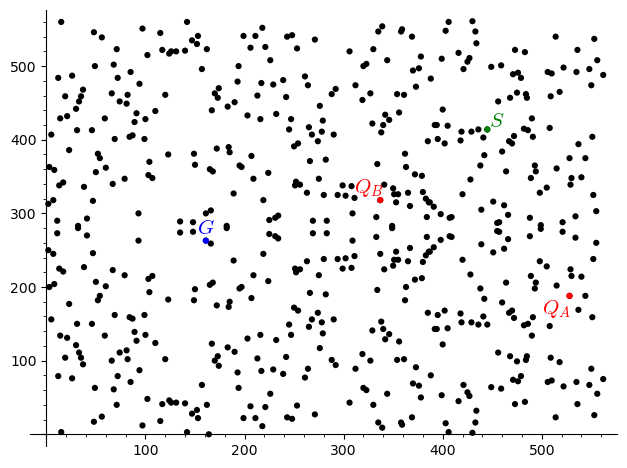
\includegraphics[height= 3in]{media/crypto.png}
    \captionof{figure}{The Elliptic-Curve Diffie-Helman exchange between Alice and Bob}
    \label{fig:crypto}
\end{figure}
\section{Future Directions} \label{sec:future}
In this section, we provide the reader with further areas of elliptic curves to investiage.

\begin{question}
    How would our results change if elliptic curves had quadratic terms in $x$? In order to answer this question, we should study the \emph{Weirtrass} form of elliptic curves \cite{cassels_1991}.
\end{question}
\begin{question}
    Describe the elements on an elliptic curve of order $2$. What would they look like geometrically?
\end{question}
\bibliographystyle{abbrv}
\bibliography{refs}
\appendix
\section{SAGE Code to Operate on Elliptic Curves}
\label{sec:code}
The following is the code in SAGE used to generate the original example in Section \ref{sec:applications}.
\begin{lstlisting}
    # define the elliptic curve
    E = EllipticCurve(GF(563), [1, -3])
    # plot the curve
    P = E.plot(pointsize = 20, color = 'black')
    # generator
    G = (161, 263)
    # plot and label the generator
    P += point(G, color = 'blue', size = 20)
    P += text(r"$G$", (161.1, 280), color='blue', fontsize=15)
    # define private keys 
    dA = 13410
    dB = 43191
    # perform operations
    Gp = E([161, 263]) 
    QA = Gp * dA
    QB = Gp * dB
    # plot and label the points
    P += point((528, 188), color = 'red', size = 20)
    P += point((337, 318), color = 'red', size = 20)
    P += text(r"$Q_A$", (515, 170), color='red', fontsize=15)
    P += text(r"$Q_B$", (325, 335), color='red', fontsize=15)
    # generate shared secret
    S = QB * dA
    # plot and label shared secret
    P += point((445, 414), color = 'green', size = 20)
    P += text(r"$S$", (455, 425), color='green', fontsize=15)
    # show the plot
    P.show(xmin = -5, xmax = 565, ymin = -5, ymax = 565)
    # print the points 
    QA
    QB
    S
    # verify the secret is shared 
    QA * dB
\end{lstlisting}
\end{document}
